%%%%%%%%%%%%%%%%%%%%%%%%%%%%%%%%%%%%%%%%%%%%%%%%%%%%%%%%%%%%%%%%%%%%%%%%%%%%%%%%%%%%%%%%%%
\section{Evaluation}
%%%%%%%%%%%%%%%%%%%%%%%%%%%%%%%%%%%%%%%%%%%%%%%%%%%%%%%%%%%%%%%%%%%%%%%%%%%%%%%%%%%%%%%%%%i
\lyt{TODO EVAL QUESTIONS}
\subsection{Security: do we meet our meet security goals}
   - attack scenarios

\subsection{Performance}

We evaluate performance using three applications: WebSubmit-rs, HotCRP, and Lobsters to answer the
following two questions.
\begin{enumerate}
    \item \emph{Cost of Disguise-Related Actions}: How expensive are \sys-enabled disguise actions
(disguise application with token storage, disguise revealing, and temporary recorrelation)?
How much does latency and storage use increase when an application uses \sys
to gain disguising and post-disguise functionality?
\item \emph{Impact on Normal Application Use}: How do \sys-enabled disguise actions impact the performance of concurrently executing
application user queries?.
\end{enumerate}

\head{Latency of Disguise-Related Actions.}
\begin{figure}[h!]
    \centering
        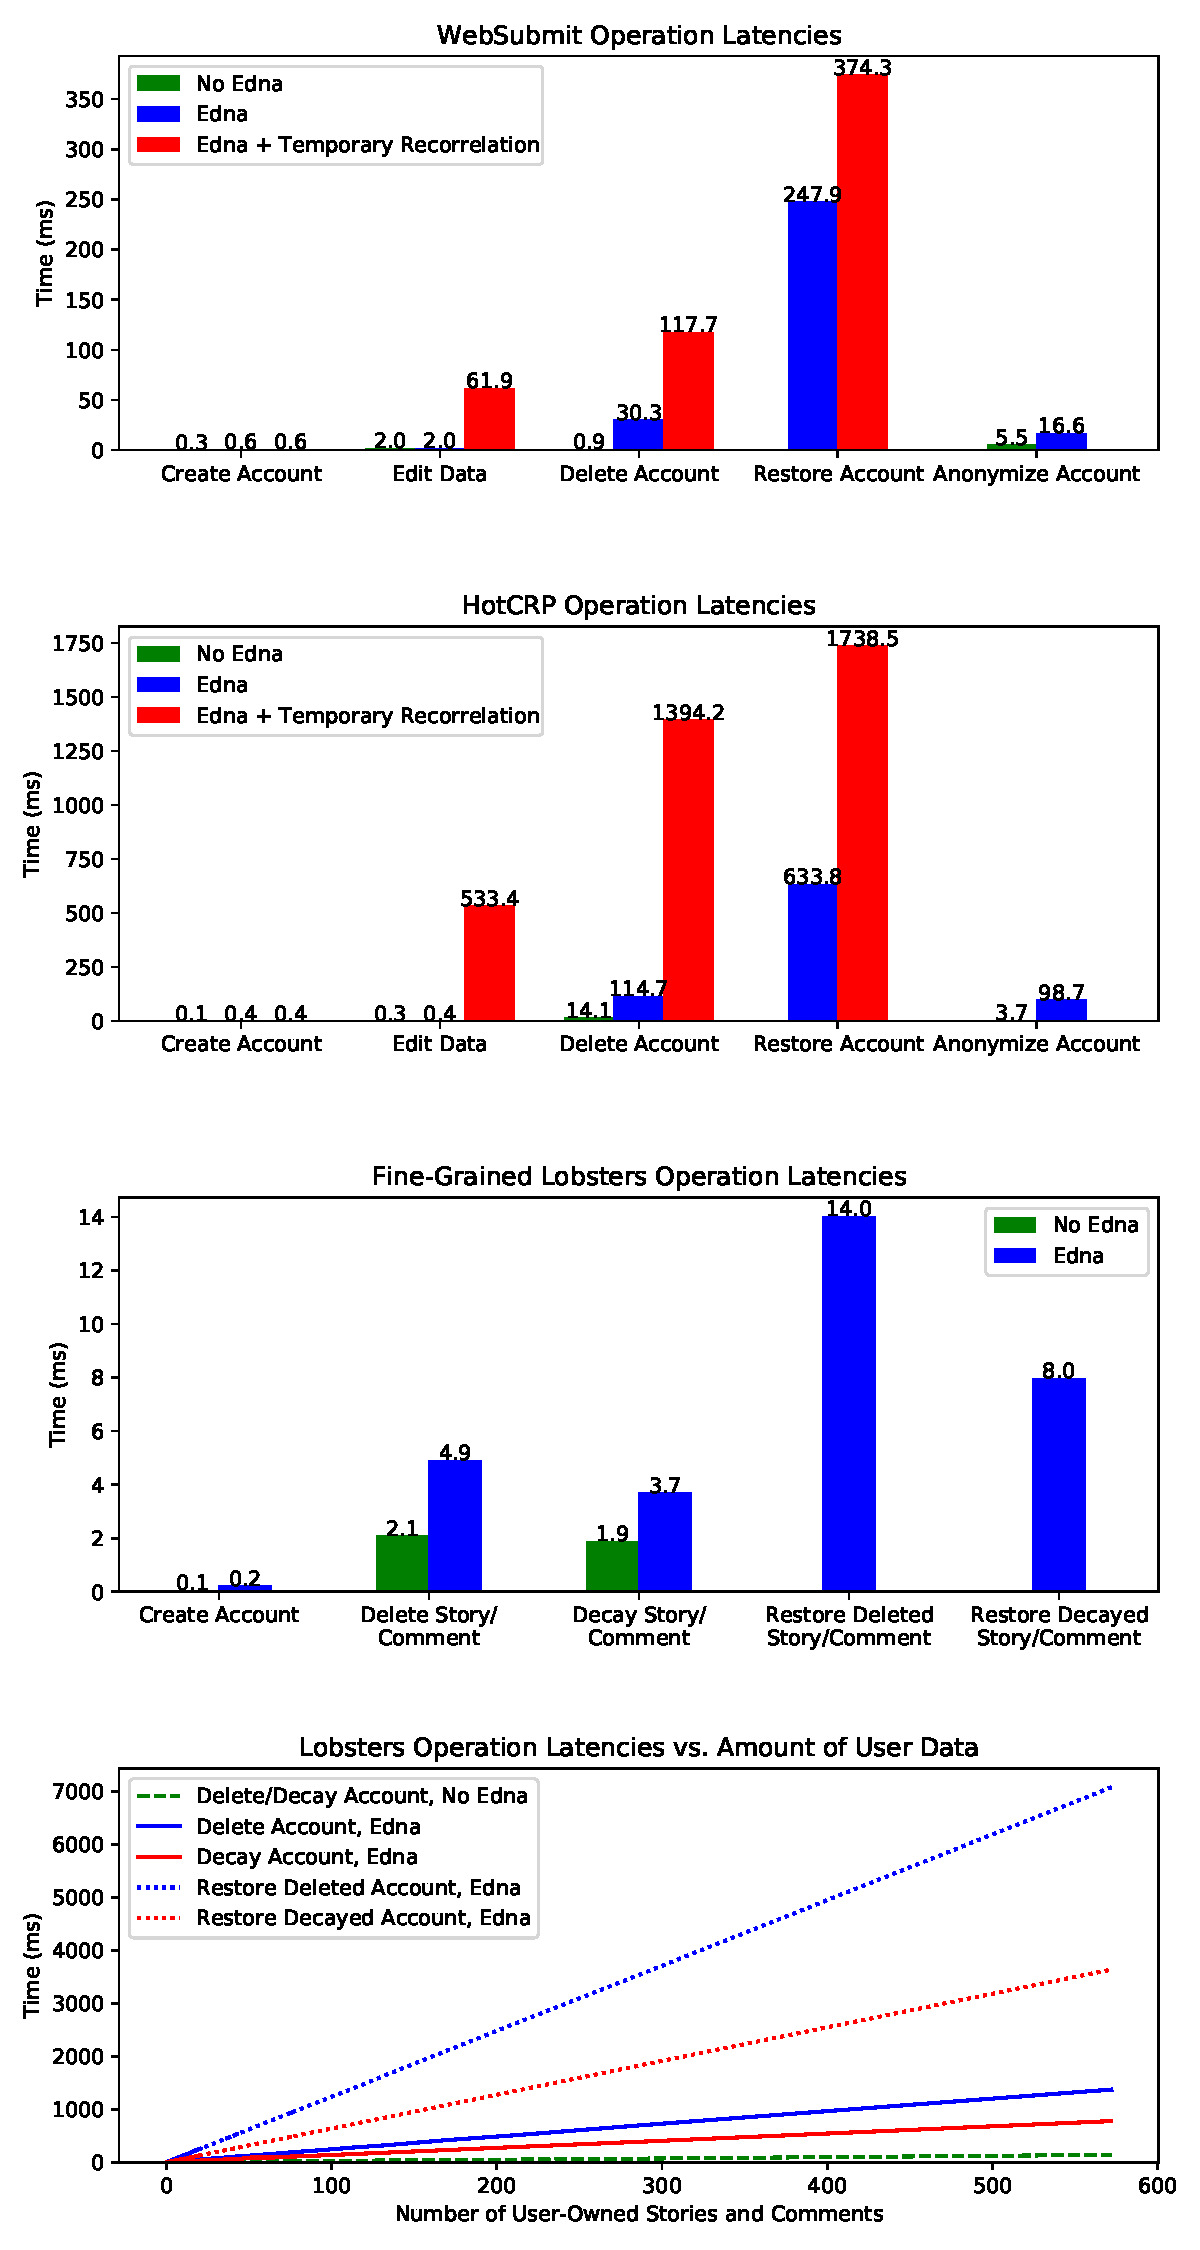
\includegraphics[width=0.5\textwidth]{figs/client_op_stats}
    \caption{Latencies of disguise-related actions when implemented manually by the application
    developer without \sys, and with \sys.
    These actions include disguise application, disguise revealing (only applicable with \sys), and
    authorized edits of anonymized data with \sys in WebSubmit and HotCRP.
    Each bar shows the median latency; the ranges indicate the 5th to 95th percentile latencies.
    } 
    \label{fig:client_opstats}
\end{figure}

\begin{table}[h!]
\begin{center}
\begin{tabular}{ c c }
\hline
\textbf{DB Op} & \textbf{Time (ms)}\\
\hline
Update DB Row & 0.1\\ 
Select DB Rows & 0.2\\
Remove DB Rows & 0.2\\
Reveal Deleted Row (DB Select + Insert) & 0.2 \\
Create + Register Principal & 0.1\\
\hline
\textbf{Crypto Op} & \textbf{Time (ms)}\\
\hline
Generate Keypair & 301\\
Encrypt SpeaksFor Token & 0.4\\
Decrypt SpeaksFor Token & 3.0\\
Encrypt Diff Token & 0.3\\
Decrypt Diff Token & 3.0\\
\end{tabular}
\end{center}
\caption{Amount of time required to run different operations required to apply and reveal disguises.}
\label{tab:opstats}
\end{table}

We measured the latency of different disguise-related actions in all three applications.

WebSubmit benchmarks measure end-to-end latency, including the time for clients to contact a (local)
server and the time for server application code (including \sys's operations) to perform these
actions and return a response.
%
WebSubmit benchmarks preopulate the database with 20 lectures, 4 questions per lecture, and 100
users.

HotCRP benchmarks run on prepopulated databases, and simulate the server-side application database
operations and how the server would invoke \sys.  An end-to-end integration with the HotCRP client
is future work; however, we imagine that modifications similar to those in WebSubmit would be
necessary.
%
HotCRP benchmarks prepopulate the database with 450 total users (50 reviewers), 450 papers (50
accepted), 4 reviews and 4 comments per paper, and a number of per-user data items (\eg paper
watches, review preferences, etc.).  

While we have an end-to-end implementation of Lobsters, we evaluate performance by generating
server-side database queries\lyt{TODO}.

%
%
Figure~\ref{fig:client_opstats} shows the cost of performing disguise-related actions with and
without \sys. We also measure the latency of actions in WebSubmit and HotCRP if composed on top of
prior anonymization, where performing these actions requires temporary recorrelation. Note that an
application \emph{must} use \sys to gain temporary recorrelation functionality, and use \sys to both
to anonymize the data in the first place and to perform the recorrelation. Thus, we do not measure
post-anonymization numbers for actions without \sys. Similarly, \sys enables account restoration or
undecay when applying account deletion or data decay, so we have no baseline latency without \sys
for account restoration or undecay.

We observe that simply using \sys without temporary recorrelation greatly increases the latency of
account deletion and anonymization.  For latency-critical tasks (such as editing data or creating an
account), \sys incurs only a slight increase in latency \lyt{Numbers}. Temporary recorrelation
after anonymization in order to perform edits or delete/restore accounts adds an additional
\lyt{Numbers} increase in latency.

We can break these costs down further into fine-grained operations shown in 
Table~\ref{tab:opstats}, since every disguise action requires some number of DB operations; if using
\sys, these actions also require cryptographic operations.

\textbf{Creating an account} with or without \sys performs a database insert. Using \sys additionally
requires registering the new user as a principal, which assigns the user a (pre-generated)
private-public key pair, stores metadata about the new principal's key in \sys's storage, and
returns the corresponding private key to the application.

\textbf{Anonymization} with or without \sys generates one pseudoprincipal per object to anonymize
(\eg answers for lectures in WebSubmit, or reviews in HotCRP). Anonymization selects the relevant answers
to anonymize, generates new pseudoprincipals, and performs DB queries to insert new pseudoprincipals
and to update objects to point to these new pseudopricipals (\eg updating foreign keys).
\sys incurs increased costs by additionally generating per-pseudoprincipal speaks-for tokens, and 
encrypting and storing these speaks-for tokens with the appropriate public keys.

\textbf{Editing data} with or without \sys simply performs update DB queries. Editing anonymized data,
however, requires temporary recorrelation to authorize the client to speak for the pseudoprincipal
associated with the data.  Most of the expense of temporary recorrelation comes from \sys decrypting
(with the client-provided decryption capability) \emph{all} speaks-for tokens at the client-provided
locator until it finds a speaks-for token linking the client to the currently-owning pseudoprincipal.
For example, if anonymization of a user account generates 20 speaks-for token ciphertexts at the same
locator, then editing anonymized data may perform up to 20 decryptions to
determine which pseudoprincipals the client can act for. This can be optimized by batching all
speaks-for tokens from one disguise into a single encrypted ciphertext, or by generating and sending
clients per-pseudoprincipal locators instead of per-disguise locators.

\textbf{Account deletion or data decay} with or without \sys performs the same DB operations to
remove, modify, or anonymize data.  \sys incurs increased costs by additionally encrypting and
inserting one diff token for each deleted or modified object, and one speaks-for token for each
anonymized object.  Account deletion post-anonymization requires \sys to perform temporary
recorrelation find data of pseudoprincipals that the user is authorized to remove along with their
account.  \sys incurs latency increases from decrypting all speaks-for tokens of the user, and from
performing the deletion or modification queries for each discovered pseudoprincipal (in addition to
the original user).

\textbf{Account restoration or undecay} is only possible with \sys. \sys decrypts a token for each
piece of modified/removed/anonymized data, and performs DB checks to ensure the data can be restored
(\eg that the corresponding lecture of an answer to reinsert still exists). If the checks pass
(which they do in this benchmark), restoration restores the data stored in the diffs. Account
restoration may also restore pseudoprincipal-associated data, which requires temporary recorrelation
to access to pseudoprincipal-associated tokens produced from the account deletion.  \sys thus
additionally decrypt speaks-for tokens for all pseudoprincipals of the user, which causes the the
increase in latency.\lyt{Numbers?}

\head{Storage Costs of Disguise-Related Actions.} 
Each generated pseudoprincipal adds an additional row to the users table in WebSubmit; \sys also
stores public-key metadata for each principal (and pseudoprincipal), and (in-memory) encrypted
ciphertexts for tokens.  Clients keep track of capabilities and locators that are emailed to them in
the form of URLs that allow for account restoration or post-anonymization editing.

\head{Impact on Normal Application Execution.} Figure~\ref{fig:concurrent} illustrates the
impacts of disguising when WebSubmit has 100 users continuously editing their lecture answers, with
250-500ms pauses between edits, and in a prepopulated database containing 2000 users, 20 lectures,
and 4 answers per lecture per user.

We imagine that a realistic normal amount of disguising would have 0 or 1 user at any point deleting
or restoring their account (in addition to the 100 editing users). With one disguiser, we observe no
increase in latency over the baseline with 0 disguisers (approximately \lyt{TODO}). 

To simulate a practical worst-case scenario, we imagine that anywhere from 10 to 25 additional
active users decide to simultaneously delete their account (\eg in response to some social media
campaign). At some later point in time, these users decide to come back and (in the worst case)
simultaneously restore their accounts. We observe that while 10 or 16 users disguising themselves at once
has minimal impact on edit latency for the 100 users, 25 users doing so causes spikes up to 2500ms.  
%
These spikes come in pairs, with the larger second spike in the pair coinciding with concurrent
revealing (and the first of the pair coinciding with disguising); revealing has greater impact due
to its higher latency and compute costs.

We imagine \sys can prevent such spikes by rate-limiting and queuing disguise actions when
necessary, in particular for non-time-sensitive disguises like GDPR-compliant account deletion.

\lyt{Include some note about how overloading the CPU with concurrent edits has some effects?}

\begin{figure}[t!]
    \centering
        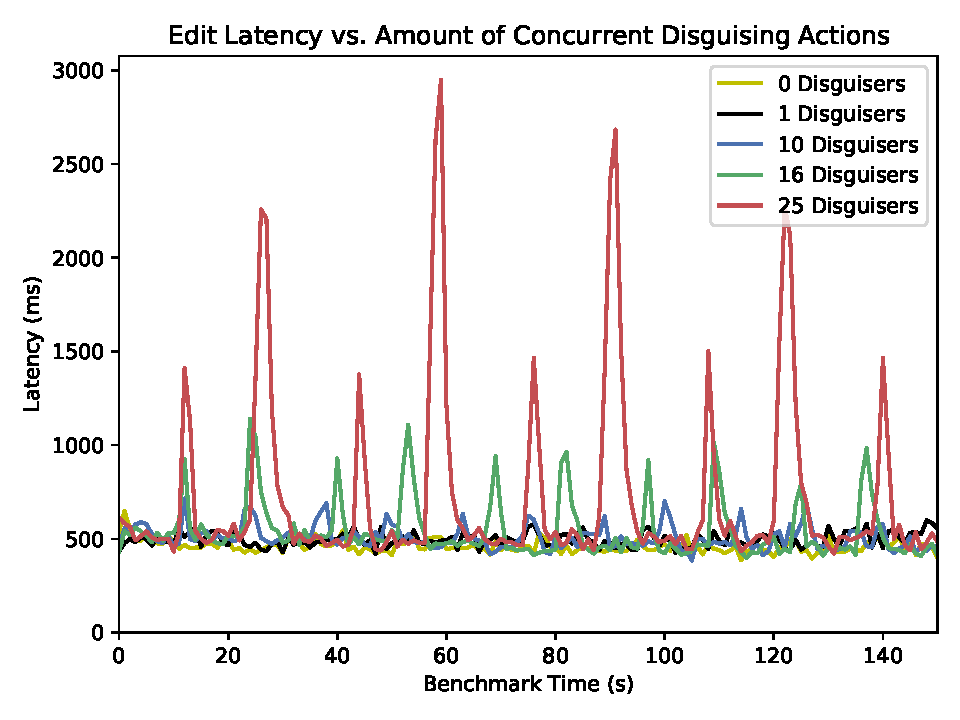
\includegraphics[width=0.5\textwidth]{figs/concurrent_results_20lec_100users}
    \caption{Impact of disguising (account deletion and revealing) on 100 users concurrently running
    normal application answer edits. Low-to-medium disguising load (<16 concurrently disguising users) has
    minimal effects on the baseline edit latency; high load (up to 25 users) causes latency spikes
    up to 2500ms.} 
    \label{fig:concurrent}
\end{figure}
